\documentclass[12 pt]{article}
\usepackage[margin = 1cm]{geometry}
\usepackage [utf8]{inputenc}
\usepackage[T2A]{fontenc}
\usepackage[russian]{babel}
\usepackage{dsfont }
\usepackage{hyperref} 
\usepackage{graphicx}
\usepackage{amsthm, amsmath, amssymb}
\usepackage{xcolor}

\begin{document}
\begin{center} 
{\bf \Large Instruction for query-function relevance labaling. } 
\end{center}

Through the annotations, we want to measure how relevant would these results be to you. 
\begin{itemize}
	\item You don't have to be absolutely certain about the correctness of the code.
	\item You might be interested in copy-pasting the code, finding a lrbrary to use or just getting some understanding about how something is implemented.
	\item You might be searching within your project (e.g. to reuse code witin your project), your company or all of GitHub.
\end{itemize}

Please annotate the results according to the following scheme:
\begin{itemize}
	\item {\bf 3: Exact match.} This seems exactly what was looking for. I would copy-paste the code and make minor adaptations or will use this functionality of the library in my code. 

	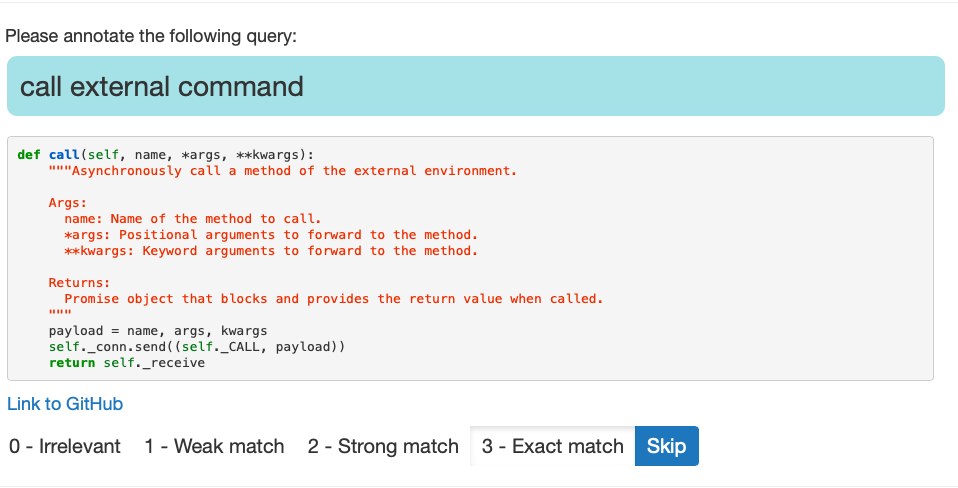
\includegraphics[width=\textwidth]{exact_match.png}
	\item {\bf 2: Strong match.} This does more or less what I was looking for. I would use the code in here as a backbone for my purpose, but I won't necessarily copy-paste it or use this library.

	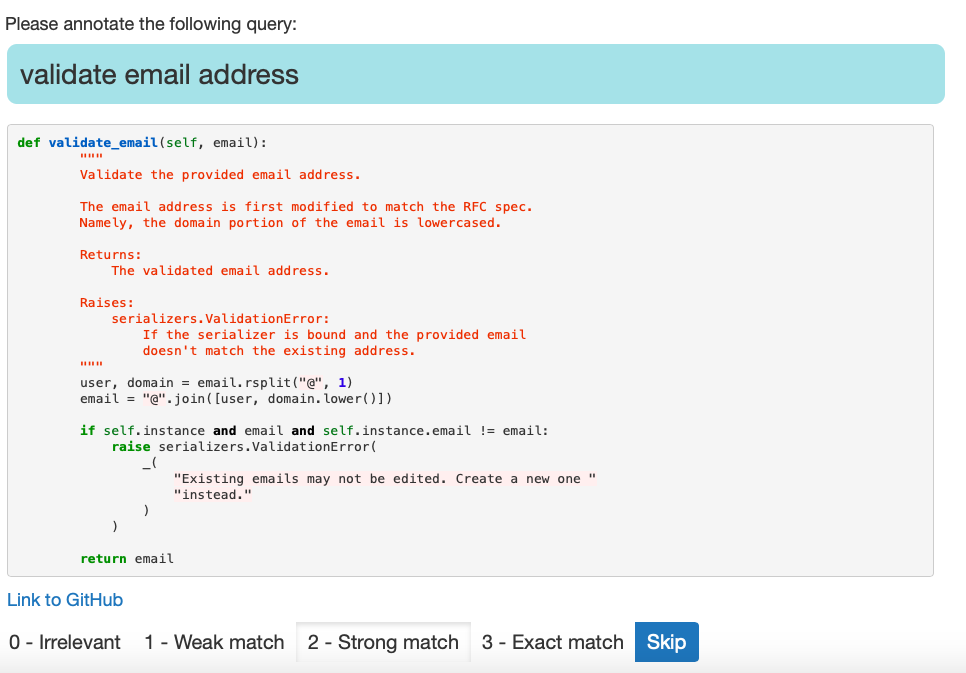
\includegraphics[width=\textwidth]{strong_match}
	\item {\bf 1: Weak match.} That's not exactly what I was looking for, but there are some useful elements/pointers to things that I would use (e.g. APIs, code structure) and can form the basis of a new query or exploration towards solving my query.

	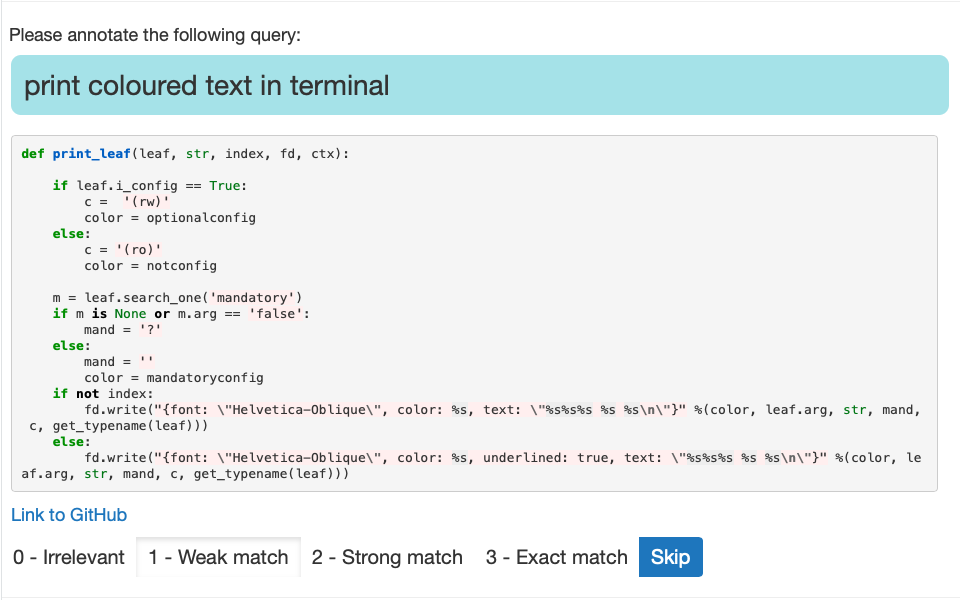
\includegraphics[width=\textwidth]{weak_match}
	\item {\bf 0: Irrelevant.} I would never want to see this tor this query.
	
	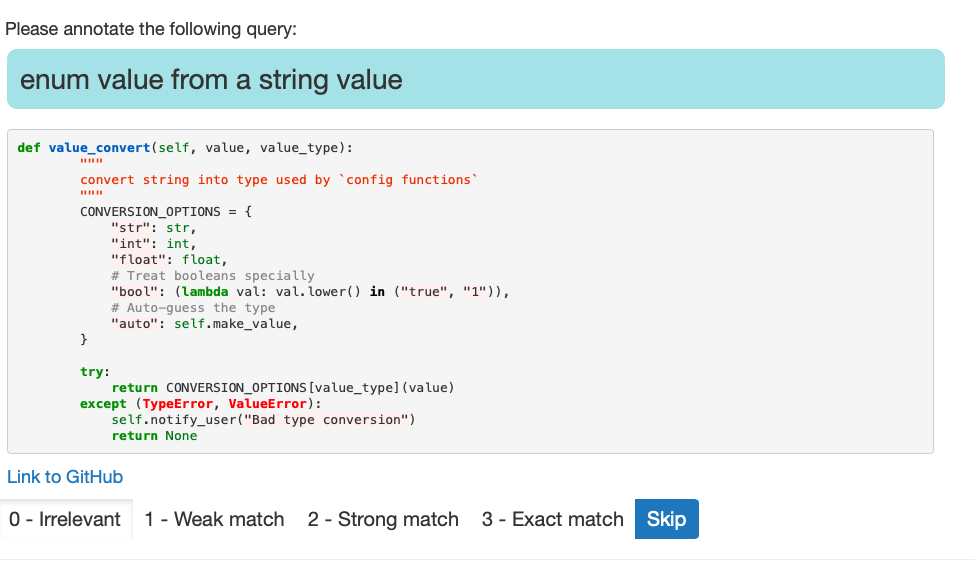
\includegraphics[width=\textwidth]{irrelevant}
\end{itemize}

\end{document}